\ifx\wholebook\relax \else
% ------------------------

\documentclass{article}
%------------------- Other types of document example ------------------------
%
%\documentclass[twocolumn]{IEEEtran-new}
%\documentclass[12pt,twoside,draft]{IEEEtran}
%\documentstyle[9pt,twocolumn,technote,twoside]{IEEEtran}
%
%-----------------------------------------------------------------------------
%%
% loading packages
%
\newif\ifpdf
\ifx\pdfoutput\undefined % We're not running pdftex
  \pdffalse
\else
  \pdftrue
\fi
%
%
\ifpdf
  \RequirePackage[pdftex,%
            CJKbookmarks,%
       bookmarksnumbered,%
              colorlinks,%
          linkcolor=blue,%
              hyperindex,%
        plainpages=false,%
       pdfstartview=FitH]{hyperref}
\else
  \RequirePackage[dvipdfm,%
             CJKbookmarks,%
        bookmarksnumbered,%
               colorlinks,%
           linkcolor=blue,%
               hyperindex,%
         plainpages=false,%
        pdfstartview=FitH]{hyperref}
  \AtBeginDvi{\special{pdf:tounicode GBK-EUC-UCS2}} % GBK -> Unicode
\fi
\usepackage{hyperref}

% other packages
%-----------------------------------------------------------------------------
\usepackage{graphicx, color}
\usepackage{CJK}
%
% for programming 
%
\usepackage{verbatim}
\usepackage{listings}


\lstdefinelanguage{Smalltalk}{
  morekeywords={self,super,true,false,nil,thisContext}, % This is overkill
  morestring=[d]',
  morecomment=[s]{"}{"},
  alsoletter={\#:},
  escapechar={!},
  literate=
    {BANG}{!}1
    {UNDERSCORE}{\_}1
    {\\st}{Smalltalk}9 % convenience -- in case \st occurs in code
    % {'}{{\textquotesingle}}1 % replaced by upquote=true in \lstset
    {_}{{$\leftarrow$}}1
    {>>>}{{\sep}}1
    {^}{{$\uparrow$}}1
    {~}{{$\sim$}}1
    {-}{{\sf -\hspace{-0.13em}-}}1  % the goal is to make - the same width as +
    %{+}{\raisebox{0.08ex}{+}}1		% and to raise + off the baseline to match -
    {-->}{{\quad$\longrightarrow$\quad}}3
	, % Don't forget the comma at the end!
  tabsize=2
}[keywords,comments,strings]

\lstloadlanguages{C++, Lisp, Smalltalk}

% ======================================================================

\def\BibTeX{{\rm B\kern-.05em{\sc i\kern-.025em b}\kern-.08em
    T\kern-.1667em\lower.7ex\hbox{E}\kern-.125emX}}

\newtheorem{theorem}{Theorem}

%
% mathematics
%
\newcommand{\be}{\begin{equation}}
\newcommand{\ee}{\end{equation}}
\newcommand{\bmat}[1]{\left( \begin{array}{#1} }
\newcommand{\emat}{\end{array} \right) }
\newcommand{\VEC}[1]{\mbox{\boldmath $#1$}}

% numbered equation array
\newcommand{\bea}{\begin{eqnarray}}
\newcommand{\eea}{\end{eqnarray}}

% equation array not numbered
\newcommand{\bean}{\begin{eqnarray*}}
\newcommand{\eean}{\end{eqnarray*}}

\RequirePackage{CJK,CJKnumb,CJKulem,CJKpunct}
% we use CJK as default environment
\AtBeginDocument{\begin{CJK*}{GBK}{song}\CJKtilde\CJKindent\CJKcaption{GB}}
\AtEndDocument{\clearpage\end{CJK*}}

%
% loading packages
%
\newif\ifpdf
\ifx\pdfoutput\undefined % We're not running pdftex
  \pdffalse
\else
  \pdftrue
\fi
%
%
\ifpdf
  \RequirePackage[pdftex,%
       bookmarksnumbered,%
              colorlinks,%
          linkcolor=blue,%
              hyperindex,%
        plainpages=false,%
       pdfstartview=FitH]{hyperref}
\else
  \RequirePackage[dvipdfm,%
        bookmarksnumbered,%
               colorlinks,%
           linkcolor=blue,%
               hyperindex,%
         plainpages=false,%
        pdfstartview=FitH]{hyperref}
\fi
\usepackage{hyperref}

% other packages
%-----------------------------------------------------------------------------
\usepackage{graphicx, color}
%
% for programming 
%
\usepackage{verbatim}
\usepackage{listings}
\usepackage{algorithmic} %for pseudocode
\usepackage{algorithm}


\lstdefinelanguage{Smalltalk}{
  morekeywords={self,super,true,false,nil,thisContext}, % This is overkill
  morestring=[d]',
  morecomment=[s]{"}{"},
  alsoletter={\#:},
  escapechar={!},
  literate=
    {BANG}{!}1
    {UNDERSCORE}{\_}1
    {\\st}{Smalltalk}9 % convenience -- in case \st occurs in code
    % {'}{{\textquotesingle}}1 % replaced by upquote=true in \lstset
    {_}{{$\leftarrow$}}1
    {>>>}{{\sep}}1
    {^}{{$\uparrow$}}1
    {~}{{$\sim$}}1
    {-}{{\sf -\hspace{-0.13em}-}}1  % the goal is to make - the same width as +
    %{+}{\raisebox{0.08ex}{+}}1		% and to raise + off the baseline to match -
    {-->}{{\quad$\longrightarrow$\quad}}3
	, % Don't forget the comma at the end!
  tabsize=2
}[keywords,comments,strings]

\lstloadlanguages{C++, Lisp, Haskell, Python, Smalltalk}

% ======================================================================

\def\BibTeX{{\rm B\kern-.05em{\sc i\kern-.025em b}\kern-.08em
    T\kern-.1667em\lower.7ex\hbox{E}\kern-.125emX}}

\newtheorem{theorem}{Theorem}

%
% mathematics
%
\newcommand{\be}{\begin{equation}}
\newcommand{\ee}{\end{equation}}
\newcommand{\bmat}[1]{\left( \begin{array}{#1} }
\newcommand{\emat}{\end{array} \right) }
\newcommand{\VEC}[1]{\mbox{\boldmath $#1$}}

% numbered equation array
\newcommand{\bea}{\begin{eqnarray}}
\newcommand{\eea}{\end{eqnarray}}

% equation array not numbered
\newcommand{\bean}{\begin{eqnarray*}}
\newcommand{\eean}{\end{eqnarray*}}




\setcounter{page}{1}

\begin{document}

%--------------------------

% ================================================================
%                 COVER PAGE
% ================================================================

\title{Radix tree, Trie and Patricia}

\author{Larry~LIU~Xinyu
\thanks{{\bfseries Larry LIU Xinyu } \newline
  Email: liuxinyu95@gmail.com \newline}
  }

\maketitle
\fi

\markboth{Radix tree, Trie and Patricia}{Elementary algorithms}

\ifx\wholebook\relax
\chapter{Radix tree, Trie and Patricia}
\numberwithin{Exercise}{chapter}
\fi

%{\bfseries Corresponding Author:} Larry LIU Xinyu


% ================================================================
%                 Introduction
% ================================================================
\section{Introduction}
\label{introduction}
\index{Radix tree}

The binary trees introduced so far store information in nodes. It's
possible to store the information in edges.
Radix trees like Trie and Patricia are important data structures in
information retrieving and manipulating.
They were invented in 1960s. And are widely used in
compiler design\cite{okasaki-int-map}, and bio-information area, such as
DNA pattern matching \cite{wiki-suffix-tree}.

\begin{figure}[htbp]
  \centering
  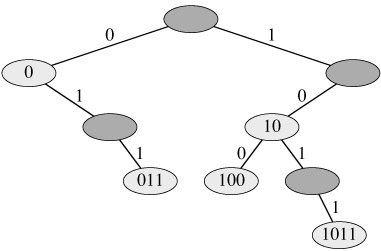
\includegraphics[scale=0.4]{img/radix-tree.ps}
  \caption{Radix tree.} \label{fig:radix-tree}
\end{figure}

Figure \ref{fig:radix-tree} shows a radix tree\cite{CLRS}. It contains the
strings of bit 1011, 10, 011, 100 and 0. When searching a key $k=(b_0b_1...b_n)_2$, we
take the first bit $b_0$ (MSB from left), check if it is 0 or 1, if it
is 0, we turn left; and turn right for 1. Then we take the second bit and
repeat this search till either meet a leaf or finish all n bits.

The radix tree needn't store keys in node at all. The
information is represented by edges. The nodes marked with keys
in the above figure are only for illustration purpose.

It is very natural to come to the idea `is it possible to represent
key in integer instead of string?' Because integer can be written in
binary format, such approach can save spaces. Another advantage is
that the speed is fast because we can use bit-wise manipulation in
most programming environment.

% ================================================================
%                 Int Trie
% ================================================================
\section{Integer Trie}
\label{int-trie}
\index{Integer trie}

The data structure shown in figure \ref{fig:radix-tree} is
often called as \emph{binary trie}.
Trie is invented by Edward Fredkin. It comes from ``retrieval'', pronounce
as /'tri:/ by the inventor, while it is pronounced /'trai/ ``try''
by other authors \cite{wiki-trie}. Trie is also called prefix tree.
A binary
trie is a special binary tree in which the placement of each key is controlled by
its bits, each 0 means ``go left'' and each 1 means ``go
right''\cite{okasaki-int-map}.

Because integers can be represented in binary format, it is
possible to store integer keys rather than 0, 1 strings. When insert an
integer as the new key to the trie, we change it to binary form, then examine
the first bit, if it is 0, we recursively
insert the rest bits to the left sub tree; otherwise if it is 1, we insert
into the right sub tree.

There is a problem when treat the key as integer. Consider a binary
trie shown in figure \ref{fig:big-endian-trie}. If represented in
0, 1 strings, all the three keys are different. But they are identical when
turn into integers. Where should we insert decimal 3, for example, to the trie?

\begin{figure}[htbp]
  \centering
  \includegraphics[scale=0.4]{img/big-endian-trie.ps}
  \caption{A big-endian trie.} \label{fig:big-endian-trie}
\end{figure}

One approach is to treat all the prefix zero as effective bits.
Suppose the integer is represented with 32-bits, If we want to insert key 1,
it ends up with a tree of 32 levels.
There are 31 nodes, each only has the left sub tree. the last node only has
the right sub tree. It is very inefficient in terms of space.

Okasaki shows a method to solve this problem in \cite{okasaki-int-map}. Instead of
using big-endian integer, we can use the little-endian integer to represent key.
Thus decimal integer 1 is represented as binary 1. Insert it to the empty binary
trie, the result is a trie with a root and a right leaf.
There is only 1 level. decimal 2 is represented as 01, and decimal 3 is $(11)_2$
in little-endian binary format. There is no need to add
any prefix 0, the position in the trie is uniquely determined.

%=========================================================================
%       Definition of integer trie
%=========================================================================
\subsection{Definition of integer Trie}
In order to define the little-endian binary trie, we can reuse the structure
of binary tree.
A binary trie node is either empty, or a branch node. The branch
node contains a left child, a right node, and optional value as
satellite data.
The left sub tree is encoded as 0 and the right sub tree
is encoded as 1.

The following example Haskell code defines the trie algebraic data type.

\lstset{language=Haskell}
\begin{lstlisting}
data IntTrie a = Empty
               | Branch (IntTrie a) (Maybe a) (IntTrie a)
\end{lstlisting}

Below is another example definition in Python.

\lstset{language=Python}
\begin{lstlisting}
class IntTrie:
    def __init__(self):
        self.left = self.right = None
        self.value = None
\end{lstlisting}


% ================================================================
%               Insertion of integer trie
% ================================================================
\subsection{Insertion}
\index{Integer trie!insert}

Since the key is little-endian integer, when insert a key, we take the
bit one by one from the right most.
If it is 0, we go to the left, otherwise go to the right
for 1. If the child is empty, we need create a new node, and repeat this to
the last bit of the key.

%\begin{algorithm}
\begin{algorithmic}[1]
\Function{Insert}{$T, k, v$}
  \If{$T =$ NIL}
    \State $T \gets$ \Call{Empty-Node}{}
  \EndIf
  \State $p \gets T$
  \While{$k \neq 0$}
    \If{\Call{Even?}{$k$}}
      \If{\Call{Left}{$p$} = NIL}
        \State \Call{Left}{$p$} $\gets$ \Call{Empty-Node}{}
      \EndIf
      \State $p \gets$ \Call{Left}{$p$}
    \Else
      \If{\Call{Right}{$p$} = NIL}
        \State \Call{Right}{$p$} $\gets$ \Call{Empty-Node}{}
      \EndIf
      \State $p \gets$ \Call{Right}{$p$}
    \EndIf
    \State $k \gets \lfloor k/2 \rfloor$
  \EndWhile
  \State \Call{Data}{$p$} $\gets v$
  \State \Return $T$
\EndFunction
\end{algorithmic}
%\end{algorithm}

This algorithm takes 3 arguments, a Trie $T$, a key $k$, and the satellite
date $v$. The following Python example code implements the insertion algorithm.
The satellite data is optional, it is empty by default.

\lstset{language=Python}
\begin{lstlisting}
def trie_insert(t, key, value = None):
    if t is None:
        t = IntTrie()
    p = t
    while key != 0:
        if key & 1 == 0:
            if p.left is None:
                p.left = IntTrie()
            p = p.left
        else:
            if p.right is None:
                p.right = IntTrie()
            p = p.right
        key = key>>1
    p.value = value
    return t
\end{lstlisting}

Figure \ref{int-trie} shows a trie which is created by inserting
pairs of key and value
\{$ 1 \rightarrow a, 4 \rightarrow b, 5 \rightarrow c, 9 \rightarrow d$\}
to the empty trie.

\begin{figure}[htbp]
  \centering
  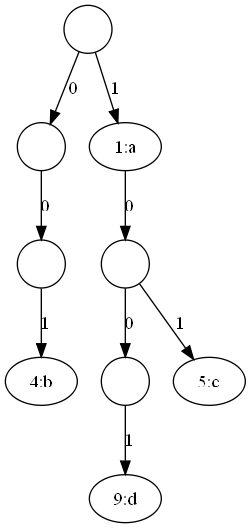
\includegraphics[scale=0.5]{img/int-trie.ps}
  \caption{A little-endian integer binary trie for the map
          \{$ 1 \rightarrow a, 4 \rightarrow b, 5 \rightarrow c, 9 \rightarrow d$\}.}
  \label{fig:int-trie}
\end{figure}

Because the definition of the integer trie is recursive, it's nature to define
the insertion algorithm recursively. If the left-most bit is 0, it
means that the key to be inserted is even, we recursively insert
to the left child, otherwise if the bit is 1, the key is odd number, the recursive
insertion is applied to the right child. we next divide the key by 2 to get
rid of the left-most bit. For trie $T$,
denote the left and right children as $T_l$ and $T_r$ respectively.
Thus $T = (T_l, d, T_r)$, where $d$ is the optional satellite data.
if $T$ is empty, $T_l$, $T_r$ and $d$ are defined as empty as well.

\be
insert(T, k, v) = \left \{
  \begin{array}
  {r@{\quad:\quad}l}
  (T_l, v, T_r) & k = 0 \\
  (insert(T_l, k / 2, v), d, T_r) & even(k) \\
  (T_l, d, insert(T_r, \lfloor k / 2 \rfloor, v)) & otherwise
  \end{array}
\right.
\ee

If the key to be inserted already exists, this algorithm just
overwrites the previous stored data. It can be replaced with
other alternatives, such as storing data as with linked-list etc.

The following Haskell example program implements the insertion
algorithm.

\lstset{language=Haskell}
\begin{lstlisting}
insert t 0 x = Branch (left t) (Just x) (right t)
insert t k x | even k = Branch (insert (left t) (k `div` 2) x) (value t) (right t)
             | otherwise = Branch (left t) (value t) (insert (right t) (k `div` 2) x)

left (Branch l _ _) = l
left Empty = Empty

right (Branch _ _ r) = r
right Empty = Empty

value (Branch _ v _) = v
value Empty = Nothing
\end{lstlisting}

For a given integer $k$ with $m$ bits in binary, the insertion algorithm
reuses $m$ levels. The performance is bound to $O(m)$ time.

% ================================================================
%               Look up in integer binary trie
% ================================================================
\subsection{Look up}
\index{Integer trie!look up}

To look up key $k$ in the little-endian integer binary trie. We take each
bit of $k$ from the left (LSB), then go left if this bit is 0, otherwise,
we go right. The looking up completes when all bits are consumed.

\begin{algorithmic}[1]
\Function{Lookup}{$T, k$}
  \While{$x \neq 0 \land T \neq $NIL}
    \If{ \Call{Even?}{$x$} }
      \State $T \gets$ \Call{Left}{$T$}
    \Else
      \State $T \gets$ \Call{Right}{$T$}
    \EndIf
    \State $k \gets \lfloor k/2 \rfloor$
  \EndWhile
  \If{$T \neq $ NIL}
    \State \Return \Call{Data}{$T$}
  \Else
    \State \Return not found \EndIf
\EndFunction
\end{algorithmic}

Below Python example code uses bit-wise operation to implements the
looking up algorithm.

\lstset{language=Python}
\begin{lstlisting}
def lookup(t, key):
    while key != 0 and (t is not None):
        if key & 1 == 0:
            t = t.left
        else:
            t = t.right
        key = key>>1
    if t is not None:
        return t.value
    else:
        return None
\end{lstlisting}

Looking up can also be define in recursive manner. If the tree is
empty, the looking up fails; If $k=0$, the satellite data is the result
to be found; If the last bit is 0, we recursively look up the
left child; otherwise, we look up the right child.

\be
lookup(T, k) =  \left \{
  \begin{array}
  {r@{\quad:\quad}l}
  \Phi & T = \Phi \\
  d & k = 0 \\
  lookup(T_l, k / 2) & even(k) \\
  lookup(T_r, \lfloor k / 2 \rfloor) & otherwise
  \end{array}
\right.
\ee

The following Haskell example program implements the recursive
look up algorithm.

\lstset{language=Haskell}
\begin{lstlisting}
search Empty k = Nothing
search t 0 = value t
search t k = if even k then search (left t) (k `div` 2)
             else search (right t) (k `div` 2)
\end{lstlisting}

The looking up algorithm is bound to $O(m)$ time, where $m$ is the
number of bits for a given key.

% ================================================================
%               Int Patricia
% ================================================================
\section{Integer Patricia}
\label{int-patricia}
\index{Integer Patricia}
\index{Integer prefix tree}

Trie has some drawbacks. It wastes a lot of
spaces. Note in figure \ref{int-trie}, only leafs store the real data.
Typically, the integer binary trie contains many nodes only have one child.
One improvement idea is to compress the chained nodes together.
Patricia is such a data structure invented by
Donald R. Morrison in 1968. Patricia means practical algorithm to retrieve information coded
in alphanumeric\cite{patricia-morrison}. It is another kind of
prefix tree.

Okasaki gives implementation of integer Patricia in \cite{okasaki-int-map}.
If we merge the chained nodes which have only one child together in figure \ref{fig:int-trie},
We can get a Patricia as shown in figure \ref{fig:little-endian-patricia}.

\begin{figure}[htbp]
  \centering
  \includegraphics[scale=0.5]{img/little-endian-patricia.ps}
  \caption{Little endian Patricia for the map
     \{$ 1 \rightarrow a, 4 \rightarrow b, 5 \rightarrow c, 9 \rightarrow d$\}.}
  \label{fig:little-endian-patricia}
\end{figure}

From this figure, we can find that the key for the sibling nodes is the
longest common prefix for them.
They branches out at certain bit. Patricia saves a lot of spaces compare
to trie.

Different from integer trie, using the big-endian integer in Patricia
doesn't cause the padding zero problem mentioned
in section \ref{int-trie}. All zero bits before MSB are omitted to save
space. Okasaki lists some significant advantages
of big-endian Patricia\cite{okasaki-int-map}.

% ================================================================
%                 Definition of int patricia tree
% ================================================================
\subsection{Definition}

Integer Patricia tree is a special kind of binary tree. It is either
empty or is a node. There are two different types of node.

\begin{itemize}
\item It can be a leaf contains integer key and optional satellite data;
\item or a branch node, contains the left and the right children. The
two children shares the longest common prefix bits for their keys.
For the left child, the next bit of the key is zero, while the next
bit is one for the right child.
\end{itemize}

The following Haskell example code defines Patricia accordingly.

\lstset{language=Haskell}
\begin{lstlisting}
type Key = Int
type Prefix = Int
type Mask = Int

data IntTree a = Empty
               | Leaf Key a
               | Branch Prefix Mask (IntTree a) (IntTree a)
\end{lstlisting}

In order to tell from which bit the left and right children differ, a
mask is recorded in the branch node. Typically, a mask is power of 2,
like $2^n$ for some non-negative integer $n$, all
bits being lower than $n$ don't belong to the common prefix.

The following Python example code defines Patricia as well as
some auxiliary functions.

\lstset{language=Python}
\begin{lstlisting}
class IntTree:
    def __init__(self, key = None, value = None):
        self.key = key
        self.value = value
        self.prefix = self.mask = None
        self.left = self.right = None

    def set_children(self, l, r):
        self.left = l
        self.right = r

    def replace_child(self, x, y):
        if self.left == x:
            self.left = y
        else:
            self.right = y

    def is_leaf(self):
        return self.left is None and self.right is None

    def get_prefix(self):
        if self.prefix is None:
            return self.key
        else:
            return self.prefix
\end{lstlisting}


% ================================================================
%                 Insertion of int patricia tree
% ================================================================
\subsection{Insertion}
\index{Integer Patricia!insert}
When insert a key, if the tree is empty,
we can just create a leaf node with the given key and satellite data,
as shown in figure \ref{fig:int-patricia-insert-a}).

\begin{figure}[htbp]
  \centering
  \includegraphics[scale=1]{img/int-patricia-insert-a.ps}
  \caption{Left: the empty tree; Right: After insert key 12.}
  \label{fig:int-patricia-insert-a}
\end{figure}

If the tree is just a singleton leaf node $x$, we can create a new leaf $y$,
put the key and data into it. After that, we need create a new branch
node, and set $x$ and $y$ as the two children.
In order to determine if the $y$ should be the left or right node, we need
find the longest common prefix of $x$ and $y$. For example if $key(x)$
is 12 ($(1100)_2$ in binary), $key(y)$ is 15 ($(1111)_2$ in binary), then the longest
common prefix is $(11oo)_2$. Where $o$ denotes the bits we don't care about.
We can use another integer to mask those bits.
In this case, the mask number is 4 (100 in binary).
The next bit after the longest common prefix presents $2^1$. This bit is
0 in $key(x)$, while it is 1 in $key(y)$. We should set $x$ as the left
child and $y$ as the right child. Figure \ref{fig:int-patricia-insert-b}
shows this example.

\begin{figure}[htbp]
  \centering
  \includegraphics[scale=1]{img/int-patricia-insert-b.ps}
  \caption{Left: A tree with singleton leaf 12; Right: After insert key 15.}
  \label{fig:int-patricia-insert-b}
\end{figure}

In case the tree is neither empty, nor a singleton leaf, we need
firstly check if the key to be inserted matches the longest common
prefix recorded in the root.
Then recursively insert the key to the left or the right child
according to the next bit of the common prefix.
For example, if insert key 14 ($(1110)_2$ in binary) to the result tree
in figure \ref{fig:int-patricia-insert-b}, since the common prefix is
$(11oo)_2$, and the next bit (the bit of $2^1$) is 1, we need recursively
insert to the right child.

If the key to be inserted doesn't match the longest
common prefix stored in the root, we need branch a new leaf
out. Figure \ref{fig:int-patricia-insert-c} shows these two different cases.

\begin{figure}[htbp]
  \centering
  \subfloat[Insert key 14. It matches the longest common prefix $(1100)_2$; 14 is then recursively inserted to the right sub tree.]{\includegraphics[scale=0.5]{img/int-patricia-insert-c.ps}}\\
  \subfloat[Insert key 5. It doesn't match the longest common prefix $(1100)_2$, a new leaf is branched out.]{\includegraphics[scale=0.5]{img/int-patricia-insert-d.ps}}
  \caption{Insert key to branch node.}
  \label{fig:int-patricia-insert-c}
\end{figure}

For a given key $k$ and value $v$, denote $(k, v)$ is the leaf node. For branch
node, denote it in form of $(p, m, T_l, T_r)$, where $p$ is the longest common
prefix, $m$ is the mask, $T_l$ and $T_r$ are the left and right children.
Summarize the above cases, the insertion algorithm can be defined as the
following.

\be
insert(T, k, v) = \left \{
  \begin{array}
  {r@{\quad:\quad}l}
  (k, v) & T = \Phi \lor T = (k, v') \\
  join(k, (k, v), k', T) & T = (k', v') \\
  (p, m, insert(T_l, k, v), T_r) & T = (p, m, T_l, T_r), match(k, p, m), zero(k, m) \\
  (p, m, T_l, insert(T_r, k, v)) & T = (p, m, T_l, T_r), match(k, p, m), \lnot zero(k, m) \\
  join(k, (k, v), p, T) & T = (p, m, T_l, T_r), \lnot match(k, p, m)
  \end{array}
\right.
\ee

The first clause deals with the edge cases, that either $T$ is empty or
it is a leaf node with the same key. The algorithm overwrites the previous
value for the later case.

The second clause handles the case that $T$ is a leaf node, but with different
key. Here we need branch out another new leaf. We need extract the longest
common prefix, and determine which leaf should be set as the left, and
which should be set as the right child. Function $join(k_1, T_1, K_2, T_2)$
does this work. We'll define it later.

The third clause deals with the case that $T$ is a branch node, the
longest common prefix matches the key to be inserted, and the next
bit to the common prefix is zero. Here we need recursively insert
to the left child.

The fourth clause handles the similar case as the third clause, except
that the next bit to the common prefix is one, but not zero. We need
recursively insert to the right child.

The last clause is for the case that the key to be inserted doesn't
match the longest common prefix stored in the branch. We need branch
out a new leaf by calling the $join$ function.

We need define function $match(k, p, m)$ to test if the key $k$, has
the same prefix $p$ above the masked bits $m$.
For example, suppose the prefix stored in a branch node is
$(p_np_{n-1} ... p_i...p_0)_2$ in binary, key $k$ is
$(k_nk_{n-1} ... k_i ... k_0)_2$ in binary, and the mask is
$(100...0)_2=2^i$. They match if and only if $p_j=k_j$ for all $i \leq j \leq n$.

One solution to realize match is to test if $mask(k, m) = p$ is satisfied.
Where $mask(x, m) = \overline{m-1} \& x$, that we perform bitwise-not of $m-1$, then
perform bitwise-and with $x$.

Function $zero(k, m)$ test the next bit of the common prefix is zero.
With the help of the mask $m$, we can shift $m$ one bit to the right,
then perform bitwise and with the key.

\be
zero(k, m) = x \& shift_r(m, 1)
\ee

If the mask $m = (100..0)_2 = 2^i$, $k = (k_nk_{n-1}...k_i1...k_0)_2$,
because the bit next to $k_i$ is 1, $zero(k, m)$ returns false value;
if $k = (k_nk_{n-1}...k_i0...k_0)_2$, then the result is true.

Function $join(p_1, T_1, p_2, T_2)$ takes two different prefixes and trees.
It extracts the longest common prefix of $p_1$ and $p_2$, create a
new branch node, and set $T_1$ and $T_2$ as the two children.

\be
join(p_1, T_1, p_2, T_2) = \left \{
  \begin{array}
  {r@{\quad:\quad}l}
  (p, m, T_1, T_2) & zero(p1, m), (p, m) = LCP(p_1, p_2) \\
  (p, m, T_2, T_1) & \lnot zero(p1, m)
  \end{array}
\right.
\ee

In order to calculate the longest common prefix of $p_1$ and $p_2$,
we can firstly compute bitwise exclusive-or for them, then count
the number of bits in this result, and generate a mask $m = 2^{|xor(p_1,p_2)|}$.
The longest common prefix $p$ can be given by masking the bits with $m$
for either $p_1$ or $p_2$.

\be
p = mask(p_1, m)
\ee

The following Haskell example code implements the insertion algorithm.

\lstset{language=Haskell}
\begin{lstlisting}
import Data.Bits

insert t k x
   = case t of
       Empty -> Leaf k x
       Leaf k' x' -> if k==k' then Leaf k x
                     else join k (Leaf k x) k' t -- t@(Leaf k' x')
       Branch p m l r
          | match k p m -> if zero k m
                           then Branch p m (insert l k x) r
                           else Branch p m l (insert r k x)
          | otherwise -> join k (Leaf k x) p t -- t@(Branch p m l r)

join p1 t1 p2 t2 = if zero p1 m then Branch p m t1 t2
                                else Branch p m t2 t1
    where
      (p, m) = lcp p1 p2

lcp :: Prefix -> Prefix -> (Prefix, Mask)
lcp p1 p2 = (p, m) where
    m = bit (highestBit (p1 `xor` p2))
    p = mask p1 m

highestBit x = if x == 0 then 0 else 1 + highestBit (shiftR x 1)

mask x m = (x .&. complement (m-1)) -- complement means bit-wise not.

zero x m = x .&. (shiftR m 1) == 0

match k p m = (mask k m) == p
\end{lstlisting}

The insertion algorithm can also be realized imperatively.

\begin{algorithmic}[1]
\Function{Insert}{$T, k, v$}
  \If{$T = $ NIL}
    \State $T \gets$ \Call{Create-Leaf}{$k, v$}
    \State \Return $T$
  \EndIf
  \State $y \gets T$
  \State $p \gets$ NIL
  \While{$y$ is not leaf, and \textproc{Match}($k$, \Call{Prefix}{$y$}, \Call{Mask}{$y$})}
    \State $p \gets y$
    \If{\textproc{Zero?}($k$, \Call{Mask}{$y$})}
      \State $y \gets$ \Call{Left}{$y$}
    \Else
      \State $y \gets$ \Call{Right}{$y$}
    \EndIf
  \EndWhile
  \If{$y$ is leaf, and $k = $ \Call{Key}{$y$}}
    \State \Call{Data}{$y$} $\gets v$
  \Else
    \State $z \gets$ \textproc{Branch}($y$, \Call{Create-Leaf}{$k, v$})
    \If{$p = $ NIL}
      \State $T \gets z$
    \Else
      \If{\Call{Left}{$p$} $ = y$}
        \State \Call{Left}{$p$} $\gets z$
      \Else
        \State \Call{Right}{$p$} $\gets z$
      \EndIf
    \EndIf
  \EndIf
  \State \Return $T$
\EndFunction
\end{algorithmic}

Function \textproc{Branch}($T_1, T_2$) does the similar job as what $join$ is defined.
It creates a new branch node, extracts the longest common prefix, and sets $T_1$ and
$T_2$ as the two children.

\begin{algorithmic}[1]
\Function{Branch}{$T_1, T_2$}
  \State $T \gets$ \Call{Empty-Node}{}
  \State $($ \Call{Prefix}{$T$}, \Call{Mask}{$T$} $) \gets$ \textproc{LCP}(\Call{Prefix}{$T_1$}, \Call{Prefix}{$T_2$})
  \If{\textproc{Zero?}(\Call{Prefix}{$T_1$}, \Call{Mask}{$T$})}
    \State \Call{Left}{$T$} $\gets T_1$
    \State \Call{Right}{$T$} $\gets T_2$
  \Else
    \State \Call{Left}{$T$} $\gets T_2$
    \State \Call{Right}{$T$} $\gets T_1$
  \EndIf
  \State \Return $T$
\EndFunction
\end{algorithmic}


The following Python example program implements the insertion algorithm.

\lstset{language=Python}
\begin{lstlisting}
def insert(t, key, value = None):
    if t is None:
        t = IntTree(key, value)
        return t

    node = t
    parent = None
    while(True):
        if match(key, node):
            parent = node
            if zero(key, node.mask):
                node = node.left
            else:
                node = node.right
        else:
            if node.is_leaf() and key == node.key:
                node.value = value
            else:
                new_node = branch(node, IntTree(key, value))
                if parent is None:
                    t = new_node
                else:
                    parent.replace_child(node, new_node)
            break
    return t
\end{lstlisting}

The auxiliary functions, \texttt{match}, \texttt{branch}, \texttt{lcp} etc. are given as below.

\begin{lstlisting}
def maskbit(x, mask):
    return x & (~(mask-1))

def match(key, tree):
    return (not tree.is_leaf()) and maskbit(key, tree.mask) == tree.prefix

def zero(x, mask):
    return x & (mask>>1) == 0

def lcp(p1, p2):
    diff = (p1 ^ p2)
    mask=1
    while(diff!=0):
        diff>>=1
        mask<<=1
    return (maskbit(p1, mask), mask)

def branch(t1, t2):
    t = IntTree()
    (t.prefix, t.mask) = lcp(t1.get_prefix(), t2.get_prefix())
    if zero(t1.get_prefix(), t.mask):
        t.set_children(t1, t2)
    else:
        t.set_children(t2, t1)
    return t
\end{lstlisting}

Figure \ref{fig:int-patricia-haskell-insert} shows the example Patricia created
with the insertion algorithm.

\begin{figure}[htbp]
  \centering
  \includegraphics[scale=0.6]{img/int-patricia-haskell-insert.ps}
  \caption{Insert map $1 \rightarrow x, 4 \rightarrow y, 5 \rightarrow z$ into the big-endian integer Patricia tree.}
  \label{fig:int-patricia-haskell-insert}
\end{figure}


% ================================================================
%                 Lookup in int patricia tree
% ================================================================
\subsection{Look up}
\index{Integer Patricia!look up}
Consider the property of integer Patricia tree. When look up a
key, if it has common prefix with the root,
then we check the next bit. If
this bit is zero, we recursively look up the left child;
otherwise if the bit is one, we next look up the right child.

When reach a leaf node, we can directly check if the key of the
leaf is equal to what we are looking up. This algorithm can be
described with the following pseudo code.

\begin{algorithmic}[1]
\Function{Look-Up}{$T, k$}
  \If{$T =$ NIL}
    \State \Return $NIL$ \Comment{Not found}
  \EndIf
  \While{$T$ is not leaf, and \textproc{Match}($k$, \Call{Prefix}{$T$}, \Call{Mask}{$T$})}
    \If{\textproc{Zero?}($k$, \Call{Mask}{$T$})}
      \State $T \gets$ \Call{Left}{$T$}
    \Else
      \State $T \gets$ \Call{Right}{$T$}
    \EndIf
  \EndWhile
  \If{$T$ is leaf, and \Call{Key}{$T$} $=k$}
    \State \Return \Call{Data}{$T$}
  \Else
    \State \Return $NIL$ \Comment{Not found}
  \EndIf
\EndFunction
\end{algorithmic}

Below Python example program implements the looking up algorithm.

\lstset{language=Python}
\begin{lstlisting}
def lookup(t, key):
    if t is None:
        return None
    while (not t.is_leaf()) and match(key, t):
        if zero(key, t.mask):
            t = t.left
        else:
            t = t.right
    if t.is_leaf() and t.key == key:
        return t.value
    else:
        return None
\end{lstlisting}

The looking up algorithm can also be realized in recursive approach.
If the Patricia tree $T$ is empty, or it's a singleton leaf with
different key from what we are looking up, the result is empty to
indicate not found error; If the tree is a singleton leaf, and the
key of this leaf is equal to what we are looking up, we are done.
Otherwise, $T$ is a branch node, we need check if the common
prefix matches the key to be looked up, and recursively look up
the child according to the next bit. If the common prefix doesn't
match the key, it means the key doesn't exist in the tree. We
can return empty result to indicate not found error.

\be
lookup(T, k) = \left \{
  \begin{array}
  {r@{\quad:\quad}l}
  \Phi & T = \Phi \lor (T = (k', v), k' \neq k) \\
  v & T = (k', v), k' = k \\
  lookup(T_l, k) & T = (p, m, T_l, T_r), match(k, p, m), zero(k, m) \\
  lookup(T_r, k) & T = (p, m, T_l, T_r), match(k, p, m), \lnot zero(k, m) \\
  \Phi & otherwise
  \end{array}
\right.
\ee

The following Haskell example program implements this recursive
looking up algorithm.

\lstset{language=Haskell}
\begin{lstlisting}
search t k
  = case t of
      Empty -> Nothing
      Leaf k' x -> if k==k' then Just x else Nothing
      Branch p m l r
             | match k p m -> if zero k m then search l k
                              else search r k
             | otherwise -> Nothing
\end{lstlisting}


% ================================================================
%                 Alphabetic trie
% ================================================================
\section{Alphabetic Trie}
\index{Trie}
Integer based Trie and Patricia Tree can be a good start point. Such
technical plays important role in Compiler implementation. Okasaki
pointed that the widely used Glasgow Haskell Compiler, GHC,
utilized the similar implementation for several years before
1998 \cite{okasaki-int-map}.

If we extend the key from integer to alphabetic
value, Trie and Patricia tree can be very powerful in solving
textual manipulation problems.

% ================================================================
%                 Definition of Alphabetic trie
% ================================================================
\subsection{Definition}
It's not enough to just use the left and right children to represent
alphabetic keys. Using English for example, there are 26 letters
and each can be lower or upper case. If we don't care about the case,
one solution is to limit the number of branches (children) to 26.
Some simplified ANSI C implementations of Trie are defined by using
the array of 26 letters. This can be illustrated as in Figure \ref{fig:trie-of-26}.

\begin{figure}[htbp]
  \centering
  \includegraphics[scale=0.5]{img/trie-of-26.ps}
  \caption{A Trie with 26 branches, containing key 'a', 'an', 'another', 'bool',
    'boy' and 'zoo'.}
  \label{fig:trie-of-26}
\end{figure}

Not all branch nodes contain data. For instance, in Figure \ref{fig:trie-of-26},
the root only has three non-empty branches representing letter 'a',
'b', and 'z'. Other branches such as for letter c, are all
empty. We don't show empty branches in the rest of this chapter.

If deal with case sensitive problems, or handle languages other than English,
there can be more letters than 26. The problem of dynamic size of sub
branches can be solved by using some collection data structures. Such
as Hash table or map.

A alphabetic trie is either empty or a node. There are two types of node.

\begin{itemize}
\item A leaf node don't has any sub trees;
\item A branch node contains multiple sub trees. Each sub tree is bound to a character.
\end{itemize}

Both leaf and branch may contain optional satellite data. The following Haskell
code shows the example definition.

\lstset{language=Haskell}
\begin{lstlisting}
data Trie a = Trie { value :: Maybe a
                   , children :: [(Char, Trie a)]}

empty = Trie Nothing []
\end{lstlisting}

Below ANSI C code defines the alphabetic trie. For illustration purpose only,
we limit the character set to lower case English letters, from 'a' to 'z'.

\lstset{language=C}
\begin{lstlisting}
struct Trie {
  struct Trie* children[26];
  void* data;
};
\end{lstlisting}


% ================================================================
%                 Insertion of Alphabetic trie
% ================================================================
\subsection{Insertion}
\index{Trie!insert}

When insert string as key, start from the root, we pick the character
one by one from the string, examine which child represents the character.
If the corresponding child is empty, a new empty node is created.
After that, the next character is used to select the proper grand child.

We repeat this process for all the characters, and finally store the
optional satellite data in the node we arrived at.

Below pseudo code describes the insertion algorithm.

\begin{algorithmic}[1]
\Function{Insert}{$T, k, v$}
  \If{$T = $ NIL}
    \State $T \gets $ \Call{Empty-Node}{}
  \EndIf
  \State $p \gets T$
  \For{each $c$ in $k$}
    \If{\Call{Children}{$p$}[c] = NIL}
      \State \Call{Children}{$p$}[c] $\gets$ \Call{Empty-Node}{}
    \EndIf
    \State $p \gets $ \Call{Children}{$p$}[c]
  \EndFor
  \State \Call{Data}{$p$} $\gets v$
  \State \Return $T$
\EndFunction
\end{algorithmic}

The following example ANSI C program implements the insertion algorithm.

\lstset{language=C}
\begin{lstlisting}
struct Trie* insert(struct Trie* t, const char* key, void* value){
    int c;
    struct Trie *p;
    if(!t)
        t = create_node();
    for (p = t; *key; ++key, p = p->children[c]) {
        c = *key - 'a';
        if (!p->children[c])
            p->children[c] = create_node();
    }
    p->data = value;
    return t;
}
\end{lstlisting}

Where function \texttt{create\_node} creates new empty node, with all
children initialized to empty.

\begin{lstlisting}
struct Trie* create_node(){
    struct Trie* t = (struct Trie*) malloc(sizeof(struct Trie));
    int i;
    for (i=0; i<26; ++i)
        t->children[i] = NULL;
    t->data = NULL;
    return t;
}
\end{lstlisting}


The insertion can also be realized in recursive way. Denote the
key to be inserted as $K = k_1k_2...k_n$, where $k_i$ is the $i$-th
character. $K'$ is the rest of characters except $k_1$. $v'$ is the
satellite data to be inserted.
The trie is in form $T = (v, C)$, where $v$ is the satellite
data, $C = \{(c_1, T_1), (c_2, T_2), ..., (c_m, T_m)\}$ is the
map of children. It maps from character $c_i$ to
sub-tree $T_i$. if $T$ is empty, then $C$ is also empty.

\be
insert(T, K, v') = \left \{
  \begin{array}
  {r@{\quad:\quad}l}
  (v', C) & K = \Phi \\
  (v, ins(C, k_1, K', v')) & otherwise.
  \end{array}
\right.
\ee

If the key is empty, the previous value $v$ is overwritten with
$v'$. Otherwise, we need check the children and perform
recursive insertion. This is realized in function $ins(C, k_1, K', v')$.
It examines key-sub tree pairs in $C$ one by one. Let $C'$ be
the rest of pairs except for the first one. This function
can be defined as below.

\be
ins(C, k_1, K', v') = \left \{
  \begin{array}
  {r@{\quad:\quad}l}
  \{(k_1, insert(\Phi, K', v'))\} & C = \Phi \\
  \{k_1, insert(T_1, K', v')\} \cup C' & k_1 = c_1 \\
  \{(c_1, T_1)\} \cup ins(C', k_1, K', v') & otherwise
  \end{array}
\right.
\ee

If $C$ is empty, we create a pair, mapping from character $k_1$ to
a new empty tree, and recursively insert the rest characters.
Otherwise, the algorithm locates the child which is mapped
from $k_1$ for further insertion.

The following Haskell example program implements the insertion
algorithm.

\lstset{language=Haskell}
\begin{lstlisting}
insert t []     x = Trie (Just x)  (children t)
insert t (k:ks) x = Trie (value t) (ins (children t) k ks x) where
    ins [] k ks x = [(k, (insert empty ks x))]
    ins (p:ps) k ks x = if fst p == k
                        then (k, insert (snd p) ks x):ps
                        else p:(ins ps k ks x)
\end{lstlisting}


% ================================================================
%                 Look up in Alphabetic trie
% ================================================================
\subsection{Look up}
\index{Trie!look up}

To look up a key, we also extract the character from the
key one by one. For each character, we search among the children
to see if there is a branch match this character.
If there is no such a child, the look up process terminates
immediately to indicate the not found error.
When we reach the last character of the key,
The data stored in the current node is what we are looking up.

\begin{algorithmic}[1]
\Function{Look-Up}{$T, key$}
  \If{$T = $ NIL}
    \State \Return not found
  \EndIf
  \For{each $c$ in $key$}
    \If{\Call{Children}{$T$}[$c$] = NIL}
      \State \Return not found
    \EndIf
    \State $T \gets $ \Call{Children}{$T$}[$c$]
  \EndFor
  \State \Return \Call{Data}{$T$}
\EndFunction
\end{algorithmic}

Below ANSI C program implements the look up algorithm. It returns NULL to indicate
not found error.

\lstset{language=C}
\begin{lstlisting}
void* lookup(struct Trie* t, const char* key) {
    while (*key && t && t->children[*key - 'a'])
        t = t->children[*key++ - 'a'];
    return (*key || !t) ? NULL : t->data;
}
\end{lstlisting}

The look up algorithm can also be realized in recursive manner. When
look up a key, we start from the first character.
If it is bound to some child, we then
recursively search the rest characters in that child.
Denote the trie as $T = (v, C)$, the key being searched as
$K = k_1k_2...k_n$ if it isn't empty. The first character in
the key is $k_1$, and the rest characters are denoted as $K'$.

\be
lookup(T, K) = \left \{
  \begin{array}
  {r@{\quad:\quad}l}
  v & K = \Phi \\
  \Phi & find(C, k_1) = \Phi \\
  lookup(T', K') & find(C, k_1) = T'
  \end{array}
\right.
\ee

Where function $find(C, k)$ examine the pairs of key-child one by one to check
if any child is bound to character $k$. If the list of pairs $C$ is empty,
the result is empty to indicate non-existence of such a child. Otherwise,
let $C = \{(k_1, T_1), (k_2, T_2), ..., (k_m, T_m)\}$, the first sub tree $T_1$
is bound to $k_1$; the rest of pairs are represented as $C'$. Below
equation defines the $find$ function.

\be
find(C, k) = \left \{
  \begin{array}
  {r@{\quad:\quad}l}
  \Phi & C = \Phi \\
  T_1 & k_1 = k \\
  find(C', k) & otherwise
  \end{array}
\right.
\ee

The following Haskell example program implements the trie looking up
algorithm. It uses the \texttt{find} function provided in standard library\cite{wiki-trie}.

\lstset{language=Haskell}
\begin{lstlisting}
find t [] = value t
find t (k:ks) = case lookup k (children t) of
                  Nothing -> Nothing
                  Just t' -> find t' ks
\end{lstlisting}

\begin{Exercise}
\begin{itemize}
\item Develop imperative trie by using collection data structure to manage multiple sub trees in
alphabetic trie.
\end{itemize}
\end{Exercise}

% ================================================================
%                 Alphabetic Patricia Tree
% ================================================================
\section{Alphabetic Patricia}
\index{Patricia}
\index{Prefix tree}

Similar to integer trie, alphabetic trie is not memory
efficient. We can use the same method to compress alphabetic trie to
Patricia.

% ================================================================
%                 Definition of Alphabetic Patricia Tree
% ================================================================
\subsection{Definition}

Alphabetic Patricia tree is a special prefix tree, each node contains
multiple branches. All children of a node share the longest common
prefix string. As the result, there is no node with only one child,
because it conflicts with the longest common prefix property.

If we turn the trie shown in figure \ref{fig:trie-of-26} into Patricia
by compressing all nodes which have only one child. we can get
a Patricia prefix tree as in figure \ref{fig:patricia-tree}.

\begin{figure}[htbp]
  \centering
  \includegraphics[scale=0.5]{img/patricia-tree.ps}
  \caption{A Patricia prefix tree, with keys: 'a', 'an', 'another', 'bool',
    'boy' and 'zoo'.}
  \label{fig:patricia-tree}
\end{figure}

We can modify the definition of alphabetic trie a bit to adapt it
to Patricia. The Patricia is either empty, or a node in form $T = (v, C)$.
Where $v$ is the optional satellite data; $C = \{(s_1, T_1), (s_2, T_2), ..., (s_n, T_n)\}$
is a list of pairs. Each pair contains a string $s_i$, which is bound
to a sub tree $T_i$.

The following Haskell example code defines Patricia accordingly.

\lstset{language=Haskell}
\begin{lstlisting}
type Key = String

data Patricia a = Patricia { value :: Maybe a
                           , children :: [(Key, Patricia a)]}

empty = Patricia Nothing []
\end{lstlisting}

Below Python code reuses the definition for trie to define Patricia.

\lstset{language=Python}
\begin{lstlisting}
class Patricia:
    def __init__(self, value = None):
        self.value = value
        self.children = {}
\end{lstlisting}

% ================================================================
%                 Insertion of Alphabetic Patrica Tree
% ================================================================
\subsection{Insertion}
\index{Patricia!insert}

When insert a key, $s$, if the Patricia is empty, we
create a leaf node as shown in figure \ref{fig:patricia-insert} (a).
Otherwise, we need check the children.
If there is some sub tree $T_i$ bound to the string $s_i$,
and there exists common prefix between $s_i$ and $s$, we
need branch out a new leaf $T_j$. The method is to
create a new internal branch node, bind it with the common
prefix. Then set $T_i$ as one child of this branch, and
$T_j$ as the other child. $T_i$ and $T_j$ share the common
prefix. This is shown in figure \ref{fig:patricia-insert} (b).
However, there are two special cases, because $s$ may be the prefix of $s_i$
as shown in figure \ref{fig:patricia-insert} (c). And
$s_i$ may be the prefix of $s$ as in figure \ref{fig:patricia-insert} (d).

\begin{figure}[htbp]
  \centering
  \subfloat[Insert key `boy' into the empty Patricia, the result is a leaf.]{\hspace{.2\textwidth}\includegraphics[scale=0.4]{img/patricia-insert-a.ps}\hspace{.1\textwidth}}
  \subfloat[Insert key `bool'. A new branch with common prefix `bo' is created.]{\hspace{.1\textwidth}\includegraphics[scale=0.4]{img/patricia-insert-b.ps}\hspace{.2\textwidth}} \\
  \subfloat[Insert key `an' with value $y$ into $x$ with prefix `another'.]{\hspace{.3\textwidth}\includegraphics[scale=0.4]{img/patricia-insert-c.ps}\hspace{.3\textwidth}} \\
  \subfloat[Insert `another', into the node with prefix `an'. We recursively insert key `other' to the child.]{\hspace{.3\textwidth}\includegraphics[scale=0.4]{img/patricia-insert-d.ps}\hspace{.3\textwidth}}
  \caption{Patricia insertion}
  \label{fig:patricia-insert}
\end{figure}

The insertion algorithm can be described as below.

\begin{algorithmic}[1]
\Function{Insert}{$T, k, v$}
  \If{$T = $ NIL}
   \State $T \gets$ \Call{Empty-Node}{}
  \EndIf
  \State $p \gets T$
  \Loop
    \State $match \gets$ FALSE
    \For{each $(s_i, T_i) \in$ \Call{Children}{$p$}}
      \If{$k = s_i$}
        \State \Call{Value}{$p$} $\gets v$
        \State \Return $T$
      \EndIf
      \State $c \gets$ \Call{LCP}{$k, s_i$}
      \State $k_1 \gets k - c$
      \State $k_2 \gets s_i - c$
      \If{$c \neq $ NIL}
        \State $match \gets$ TRUE
        \If{$k_2 = $ NIL} \Comment{$s_i$ is prefix of $k$}
          \State $p \gets T_i$
          \State $k \gets k_1$
          \State break
        \Else \Comment{Branch out a new leaf}
          \State \Call{Children}{$p$} $\gets$ \Call{Children}{$p$} $\cup \{$ ($c$, \Call{Branch}{$k_1, v, k_2, T_i$}) $\}$
          \State \textproc{Delete}(\Call{Children}{$p$}, $(s_i, T_i)$)
          \State \Return $T$
        \EndIf
      \EndIf
    \EndFor
    \If{$\lnot match$} \Comment{Add a new leaf}
      \State \Call{Children}{$p$} $\gets$ \Call{Children}{$p$} $\cup \{$ ($k$, \Call{Create-Leaf}{$v$}) $\}$
      \State \Return $T$
    \EndIf
  \EndLoop
  \State \Return $T$
\EndFunction
\end{algorithmic}

In the above algorithm, \textproc{LCP} function finds the longest
common prefix of two given strings, for example, string `bool' and `boy'
has the longest common prefix `bo'. The subtraction symbol '-' for
strings gives the different part of two strings. For example `bool' - `bo' = `ol'. \textproc{Branch} function creates a branch node
and updates keys accordingly.

The longest common prefix can be extracted by checking the characters in the two
strings one by one till there are two characters don't match.

\begin{algorithmic}[1]
\Function{LCP}{$A, B$}
  \State $i \gets 1 $
  \While{$i \leq |A| \land i \leq |B| \land A[i] = B[i]$}
    \State $i \gets i + 1$
  \EndWhile
  \State \Return $A[1...i-1]$
\EndFunction
\end{algorithmic}

There are two cases when branch out a new leaf. \textproc{Branch}($s_1, T_1, s_2, T_2$)
takes two different keys and two trees. If $s_1$ is empty, we are
dealing the case such as insert key `an' into a child bound to
string `another'. We set $T_2$ as the child of $T_1$. Otherwise,
we create a new branch node and set $T_1$ and $T_2$ as the two children.

\begin{algorithmic}[1]
\Function{Branch}{$s_1, T_1, s_2, T_2$}
  \If{$s_1 = \Phi$}
    \State \Call{Children}{$T_1$} $\gets$ \Call{Children}{$T_1$} $\cup \{(s_2, T_2)\}$
    \State \Return $T_1$
  \EndIf
  \State $T \gets$ \Call{Empty-Node}{}
  \State \Call{Children}{$T$} $\gets \{(s_1, T_1), (s_2, T_2)\}$
  \State \Return $T$
\EndFunction
\end{algorithmic}

The following example Python program implements the Patricia insertion algorithm.

\lstset{language=Python}
\begin{lstlisting}
def insert(t, key, value = None):
    if t is None:
        t = Patricia()
    node = t
    while True:
        match = False
        for k, tr in node.children.items():
            if key == k: # just overwrite
                node.value = value
                return t
            (prefix, k1, k2) = lcp(key, k)
            if prefix != "":
                match = True
                if k2 == "":
                    # example: insert "another" into "an", go on traversing
                    node = tr
                    key = k1
                    break
                else: #branch out a new leaf
                    node.children[prefix] = branch(k1, Patricia(value), k2, tr)
                    del node.children[k]
                    return t
        if not match: # add a new leaf
            node.children[key] = Patricia(value)
            return t
    return t
\end{lstlisting}

Where the functions to find the longest common prefix, and branch out are
implemented as below.

\begin{lstlisting}
# returns (p, s1', s2'), where p is lcp, s1'=s1-p, s2'=s2-p
def lcp(s1, s2):
    j = 0
    while j < len(s1) and j < len(s2) and s1[j] == s2[j]:
        j += 1
    return (s1[0:j], s1[j:], s2[j:])

def branch(key1, tree1, key2, tree2):
    if key1 == "":
        #example: insert "an" into "another"
        tree1.children[key2] = tree2
        return tree1
    t = Patricia()
    t.children[key1] = tree1
    t.children[key2] = tree2
    return t
\end{lstlisting}

The insertion can also be realized recursively. Start from the root,
the program checks all the children to find if there is a node matches
the key. Matching means they have the common
prefix. For duplicated keys, the program overwrites previous value.
There are also alternative solution to handle duplicated keys, such
as using linked-list etc. If there is no child matches the
key, the program creates a new leaf, and add it to the children.

For Patricia $T = (v, C)$, function $insert(T, k, v')$ inserts
key $k$, and value $v'$ to the tree.

\be
insert(T, k, v') = (v, ins(C, k, v'))
\ee

This function calls another internal function $ins(C, k, v')$.
If the children $C$ is empty, a new leaf is created; Otherwise
the children are examined one by one. Denote $C = \{(k_1, T_1), (k_2, T_2), ..., (k_n, T_n)\}$,
$C'$ holds all the prefix-sub tree pairs except for the first one.

\be
ins(C, k, v') = \left \{
  \begin{array}
  {r@{\quad:\quad}l}
  \{(k, (v', \Phi))\} & C = \Phi \\
  \{(k, (v', C_{T_1}))\} \cup C' & k_1 = k \\
  \{branch(k, v', k_1, T_1)\} \cup C' & match(k_1, k) \\
  \{(k_1, T_1)\} \cup ins(C', k, v') & otherwise
  \end{array}
\right.
\ee

The first clause deals with the edge case of empty children. A
leaf node containing $v'$ which is bound to $k$ will be
returned as the only child. The second clause overwrites
the previous value with $v'$ if there is some child bound
to the same key. Note the $C_{T_1}$ means the children of
sub tree $T_1$. The third clause branches out a new leaf
if the first child matches the key $k$. The last clause
goes on checking the rest children.

We define two keys $A$ and $B$ matching if they
have non-empty common prefix.

\be
match(A, B) = A \neq \Phi \land B \neq \Phi \land a_1 = b_1
\ee

Where $a_1$ and $b_1$ are the first characters in $A$ and $B$ if
they are not empty.

Function $branch(k_1, v, k_2, T_2)$ takes tow keys, a value
and a tree. Extract the longest common prefix $k = lcp(k_1, k_2)$,
Denote the different part as $k_1' = k_1 - k$, $k_2' = k_2 - k$.
The algorithm firstly handles the edge cases that either $k_1$ is the prefix
of $k_2$ or $k_2$ is the prefix of $k_1$. For the former case,
It creates a new node containing $v$, bind this node to $k$,
and set $(k_2', T_2)$ as the only child; For the later case,
It recursively insert $k_1'$ and $v$ to $T_2$. Otherwise,
the algorithm creates a branch node, binds it to the longest
common prefix $k$, and set two children for it. One child
is $(k_2', T_2)$, the other is a leaf node containing $v$, and
being bound to $k_1'$.

\be
branch(k_1, v, k_2, T_2) = \left \{
  \begin{array}
  {r@{\quad:\quad}l}
  (k, (v, \{(k_2', T_2)\})) & k = k_1 \\
  (k, insert(T_2, k_1', v)) & k = k_2 \\
  (k, (\Phi, \{(k_1', (v, \Phi)), (k_2', T_2)\}) & otherwise
  \end{array}
\right.
\ee

And function $lcp(A, B)$ keeps taking same characters from $A$ and $B$
one by one. Denote $a_1$ and $b_1$ as
the first characters in $A$ and $B$ if they are not empty.
$A'$ and $B'$ are the rest parts except for the first characters.

\be
lcp(A, B) = \left \{
  \begin{array}
  {r@{\quad:\quad}l}
  \Phi & A = \Phi \lor B = \Phi \lor a_1 \neq b_1 \\
  \{a_1\} \cup lcp(A', B') & a_1 = b_1
  \end{array}
\right.
\ee

The following Haskell example program implements the Patricia insertion
algorithm.

\lstset{language=Haskell}
\begin{lstlisting}
insert t k x = Patricia (value t) (ins (children t) k x) where
    ins []     k x = [(k, Patricia (Just x) [])]
    ins (p:ps) k x
        | (fst p) == k
            = (k, Patricia (Just x) (children (snd p))):ps --overwrite
        | match (fst p) k
            = (branch k x (fst p) (snd p)):ps
        | otherwise
            = p:(ins ps k x)

match x y = x /= [] && y /= [] && head x == head y

branch k1 x k2 t2
    | k1 == k
        -- ex: insert "an" into "another"
        = (k, Patricia (Just x) [(k2', t2)])
    | k2 == k
        -- ex: insert "another" into "an"
        = (k, insert t2 k1' x)
    | otherwise = (k, Patricia Nothing [(k1', leaf x), (k2', t2)])
   where
      k = lcp k1 k2
      k1' = drop (length k) k1
      k2' = drop (length k) k2

lcp [] _ = []
lcp _ [] = []
lcp (x:xs) (y:ys) = if x == y then x:(lcp xs ys) else []
\end{lstlisting}


% ================================================================
%                 Look up in Alphabetic Patrica Tree
% ================================================================
\subsection{Look up}
\index{Patricia!look up}
When look up a key, we can't examine the characters one by one
as in trie. Start from the root, we need search among the children
to see if any one is bound to a prefix of the key.
If there is such a child, we update the key by removing the prefix
part, and recursively look up the updated key in this child.
If there aren't any children bound to any prefix of the key,
the looking up fails.

\begin{algorithmic}[1]
\Function{Look-Up}{$T, k$}
  \If{$T = $ NIL}
     \State \Return not found
   \EndIf
  \Repeat
    \State $match \gets$ FALSE
    \For{$\forall (k_i, T_i) \in $ \Call{Children}{$T$}}
      \If{$k = k_i$}
        \State \Return \Call{Data}{$T_i$}
      \EndIf
      \If{$k_i$ is prefix of $k$}
        \State $match \gets$ TRUE
        \State $k \gets k - k_i$
        \State $T \gets T_i$
        \State break
      \EndIf
    \EndFor
  \Until{$\lnot match$}
  \State \Return not found
\EndFunction
\end{algorithmic}

Below Python example program implements the looking up algorithm.
It reuses the \texttt{lcp(s1, s2)} function
defined previously to test if a string is the prefix of the other.

\lstset{language=Python}
\begin{lstlisting}
def lookup(t, key):
    if t is None:
        return None
    while True:
        match = False
        for k, tr in t.children.items():
            if k == key:
                return tr.value
            (prefix, k1, k2) = lcp(key, k)
            if prefix != "" and k2 == "":
                match = True
                key = k1
                t = tr
                break
        if not match:
            return None
\end{lstlisting}

This algorithm can also be realized recursively. For Patricia in form
$T = (v, C)$, it calls another function to find among the children $C$.

\be
lookup(T, k) = find(C, k)
\ee

If $C$ is empty, the looking up fails; Otherwise, For $C = \{(k_1, T_1), (k_2, T_2), ..., (k_n, T_n)\}$, we firstly examine if $k$ is the prefix of $k_1$, if not the
recursively check the rest pairs denoted as $C'$.

\be
find(C, k) = \left \{
  \begin{array}
  {r@{\quad:\quad}l}
  \Phi & C = \Phi \\
  v_{T_1} & k = k_1 \\
  lookup(T_1, k - k_1) & k_1 \sqsubset k \\
  find(C', k) & otherwise
  \end{array}
\right.
\ee

Where $A \sqsubset B$ means string $A$ is prefix of $B$. $find$ mutually
calls $lookup$ if some child is bound to a string which is prefix of
the key.

Below Haskell example program implements the looking up algorithm.

\lstset{language=Haskell}
\begin{lstlisting}
import qualified Data.List

find t k = find' (children t) k where
    find' [] _ = Nothing
    find' (p:ps) k
          | (fst p) == k = value (snd p)
          | (fst p) `Data.List.isPrefixOf` k = find (snd p) (diff (fst p) k)
          | otherwise = find' ps k
    diff k1 k2 = drop (length (lcp k1 k2)) k2
\end{lstlisting}


% ================================================================
%                 Trie and Patrica used in Industry
% ================================================================
\section{Trie and Patricia applications}

Trie and Patricia can be used to solving some interesting problems.
Integer based prefix tree is used in compiler implementation. Some daily
used software applications have many interesting features which can be
realized with trie or Patricia. In this section, some applications are
given as examples, including, e-dictionary, word auto-completion, T9
input method etc.
The commercial implementations typically do not adopt trie or Patricia
directly. The solutions we demonstrated here are for illustration purpose
only.

\subsection{E-dictionary and word auto-completion}
\index{Auto completion}
Figure \ref{fig:e-dict} shows a screen shot of an English-Chinese E-dictionary.
In order to provide good user experience,
the dictionary searches its word library, and lists all candidate words and
phrases similar to what user has entered.

\begin{figure}[htbp]
  \centering
  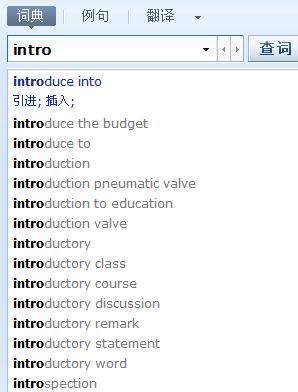
\includegraphics[scale=0.5]{img/ciba.eps}
  \caption{E-dictionary. All candidates starting with what the user input are listed.}
  \label{fig:e-dict}
\end{figure}

A E-dictionary typically contains hundreds of thousands words. It's very expensive
to performs a whole word search. Commercial software adopts complex approaches, including
caching, indexing etc to speed up this process.

Similar with e-dictionary, figure \ref{fig:word-completion} shows a popular
Internet search engine. When user input something, it provides a candidate
lists, with all items starting with what the user has entered. And these candidates
are shown in the order of popularity. The more people search, the
upper position it is in the list.

\begin{figure}[htbp]
  \centering
  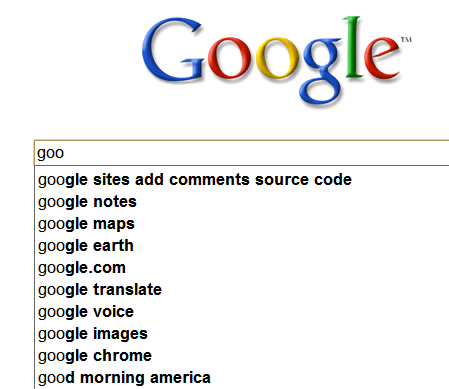
\includegraphics[scale=0.5]{img/adaptive-input.eps}
  \caption{A search engine. All candidates starting with what user input are listed.}
  \label{fig:word-completion}
\end{figure}

In both cases, the software provides a kind of word auto-completion mechanism.
In some modern IDEs, the editor can even help users to auto-complete program code.

Let's see how to implementation of the e-dictionary with trie or Patricia.
To simplify the problem, we assume the dictionary only supports English - English
information.

A dictionary stores key-value pairs, the keys are English
words or phrases, the values are the meaning described in English sentences.

We can store all the words and their meanings in a trie, but it isn't
space effective especially when there are huge amount of items. We'll use
Patricia to realize e-dictionary.

When user wants to look up word 'a', the dictionary does not only
return the meaning of 'a', but also provides a list of
candidate words, which all start with 'a', including 'abandon', 'about',
'accent', 'adam', ... Of course all these words are stored in the Patricia.

If there are too many candidates, one solution is only displaying the top 10
words, and the user can browse for more.

The following algorithm reuses the looking up defined for Patricia. When it
finds a node bound to a string which is the prefix of what we are looking for,
it expands all its children until getting $n$ candidates.

\begin{algorithmic}[1]
\Function{Look-Up}{$T, k, n$}
  \If{$T = $ NIL}
     \State \Return $\Phi$
  \EndIf
  \State $prefix \gets$ NIL
  \Repeat
    \State $match \gets$ FALSE
    \For{$\forall (k_i, T_i) \in $ \Call{Children}{$T$}}
      \If{$k$ is prefix of $k_i$}
        \State \Return \Call{Expand}{$T_i, prefix, n$}
      \EndIf
      \If{$k_i$ is prefix of $k$}
        \State $match \gets$ TRUE
        \State $k \gets k - k_i$
        \State $T \gets T_i$
        \State $prefix \gets prefix + k_i$
        \State break
      \EndIf
    \EndFor
  \Until{$\lnot match$}
  \State \Return $\Phi$
\EndFunction
\end{algorithmic}

Where function \textproc{Expand}($T, prefix, n$) picks $n$ sub trees, which
share the same prefix in $T$. It is realized as BFS (Bread-First-Search) traverse. Chapter search
explains BFS in detail.

\begin{algorithmic}[1]
\Function{Expand}{$T, prefix, n$}
  \State $R \gets \Phi$
  \State $Q \gets \{(prefix, T)\}$
  \While{$|R| < n \land |Q| > 0$}
    \State $(k, T) \gets$ \Call{Pop}{$Q$}
    \If{\Call{Data}{$T$} $\neq$ NIL}
      \State $R \gets R \cup \{(k, $ \Call{Data}{$T$} $)\}$
    \EndIf
    \For{$\forall (k_i, T_i) \in$ \Call{Children}{$T$}}
      \State \Call{Push}{$Q, (k + k_i, T_i)$}
    \EndFor
  \EndWhile
\EndFunction
\end{algorithmic}

The following example Python program implements the e-dictionary application.
When testing if a string is prefix of another one, it uses the \texttt{find}
function provided in standard string library.

\lstset{language=Python}
\begin{lstlisting}
import string

def patricia_lookup(t, key, n):
    if t is None:
        return None
    prefix = ""
    while True:
        match = False
        for k, tr in t.children.items():
            if string.find(k, key) == 0: #is prefix of
                return expand(prefix+k, tr, n)
            if string.find(key, k) ==0:
                match = True
                key = key[len(k):]
                t = tr
                prefix += k
                break
        if not match:
            return None

def expand(prefix, t, n):
    res = []
    q = [(prefix, t)]
    while len(res)<n and len(q)>0:
        (s, p) = q.pop(0)
        if p.value is not None:
            res.append((s, p.value))
        for k, tr in p.children.items():
            q.append((s+k, tr))
    return res
\end{lstlisting}

This algorithm can also be implemented recursively, if the string we
are looking for is empty, we expand all children until getting $n$
candidates. Otherwise we recursively examine the children to
find one which has prefix equal to this string.

In programming environments supporting lazy evaluation. An intuitive
solution is to expand all candidates, and take the first $n$ on
demand. Denote the Patricia prefix tree in form $T = (v, C)$,
below function enumerates all items starts with key $k$.

\be
findAll(T, k) = \left \{
  \begin{array}
  {r@{\quad:\quad}l}
  enum(C) & k = \Phi, v = \Phi \\
  \{(\Phi, v)\} \cup enum(C) & k = \Phi, v \neq \Phi \\
  find(C, k) & k \neq \Phi
  \end{array}
\right.
\ee

The first two clauses deal with the edge cases the the key is empty.
All the children are enumerated except for those with empty values.
The last clause finds child matches $k$.

For non-empty children, $C = \{(k_1, T_1), (k_2, T_2), ..., (k_m, T_m)\}$,
denote the rest pairs except for the first one as $C'$.
The enumeration algorithm can be defined as below.

\be
enum(C) = \left \{
  \begin{array}
  {r@{\quad:\quad}l}
  \Phi & C = \Phi \\
  mapAppend(k_1, findAll(T_1, \Phi)) \cup enum(C')
  \end{array}
\right.
\ee

Where $mapAppend(k, L) = \{(k + k_i, v_i)| (k_i, v_i) \in L\}$. It concatenate
the prefix $k$ in front of every key-value pair in list $L$.

Function $find(C, k)$ is defined as the following. For empty children, the
result is empty as well; Otherwise, it examines the first child $T_1$ which
is bound to string $k_1$. If $k_1$ is equal to $k$, it calls $mapAppend$ to
add prefix to the keys of all the children under $T_1$; If $k_1$ is prefix
of $k$, the algorithm recursively find all children start with $k - k_1$;
On the other hand, if $k$ is prefix of $k_1$, all children under $T_1$
are valid result. Otherwise, the algorithm by-pass the first child
and goes on find the rest children.

\be
find(C, k) = \left \{
  \begin{array}
  {r@{\quad:\quad}l}
  \Phi & C = \Phi \\
  mapAppend(k, findAll(T_1, \Phi)) & k_1 = k \\
  mapAppend(k_1, findAll(T_1, k - k_1)) & k_1 \sqsubset k \\
  findAll(T_1, \Phi) & k \sqsubset k_1 \\
  find(C', k) & otherwise
  \end{array}
\right.
\ee

Below example Haskell program implements the e-dictionary application
according to the above equations.

\lstset{language=Haskell}
\begin{lstlisting}
findAll :: Patricia a -> Key -> [(Key, a)]
findAll t [] =
    case value t of
      Nothing -> enum $ children t
      Just x  -> ("", x):(enum $ children t)
    where
      enum [] = []
      enum (p:ps) = (mapAppend (fst p) (findAll (snd p) [])) ++ (enum ps)
findAll t k = find' (children t) k where
    find' [] _ = []
    find' (p:ps) k
          | (fst p) == k
              = mapAppend k (findAll (snd p) [])
          | (fst p) `Data.List.isPrefixOf` k
              = mapAppend (fst p) (findAll (snd p) (k `diff` (fst p)))
          | k `Data.List.isPrefixOf` (fst p)
              = findAll (snd p) []
          | otherwise = find' ps k
    diff x y = drop (length y) x

mapAppend s lst = map (\p->(s++(fst p), snd p)) lst
\end{lstlisting}

In the lazy evaluation environment, the top $n$ candidates can be
gotten like $take(n, findAll(T, k))$. Appendix A has detailed definition
of $take$ function.

%=====================================
% T9
%=====================================

\subsection{T9 input method}
\index{T9}
\index{Textonym input method}

Most mobile phones around year 2000 are equipped with a key pad.
Users have quite different experience from PC when editing a short message
or email.
This is because the mobile-phone key pad, or so called ITU-T key pad has much fewer
keys than PC. Figure \ref{fig:itut-keypad} shows one example.

\begin{figure}[htbp]
  \centering
  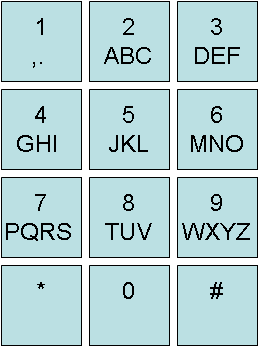
\includegraphics[scale=0.4]{img/itu-t.eps}
  \caption{an ITU-T keypad for mobile phone.}
  \label{fig:itut-keypad}
\end{figure}

There are typical two methods to input English word or phrases with ITU-T key pad.
For instance, if user wants to enter a word `home', He can press the key
in below sequence.

\begin{itemize}
\item Press key '4' twice to enter the letter 'h';
\item Press key '6' three times to enter the letter 'o';
\item Press key '6' twice to enter the letter 'm';
\item Press key '3' twice to enter the letter 'e';
\end{itemize}

Another much quicker way is to just press the following keys.

\begin{itemize}
\item Press key '4', '6', '6', '3', word `home' appears on top of the candidate list;
\item Press key '*' to change a candidate word, so word `good' appears;
\item Press key '*' again to change another candidate word, next word `gone' appears;
\item ...
\end{itemize}

Compare these two methods, we can see the second one is much easier for the end user.
The only overhead is to store a dictionary of candidate words.

Method 2 is called as `T9' input method, or predictive input method
\cite{wiki-t9}, \cite {wiki-predictive-text}. The abbreviation 'T9' stands
for 'textonym'. It start with 'T' with 9 characters. T9 input can also be
realized with trie or Patricia.

In order to provide candidate words to user, a dictionary must be prepared
in advance. Trie or Patricia can be used to store the dictionary. The
commercial T9 implementations typically use complex indexing dictionary in
both file system and cache. The realization shown here is for illustration
purpose only.

Firstly, we need define the T9 mapping, which maps from digit to candidate
characters.

\be
\begin{array}{ll}
M_{T9} = \{ & 2 \rightarrow abc, 3 \rightarrow def, 4 \rightarrow ghi, \\
           & 5 \rightarrow jkl, 6 \rightarrow mno, 7 \rightarrow pqrs, \\
           & 8 \rightarrow tuv, 9 \rightarrow wxyz \}
\end{array}
\ee

With this mapping, $M_{T9}[i]$ returns the corresponding characters for digit $i$.

Suppose user input digits $D = d_1d_2...d_n$, If $D$ isn't empty, denote the
rest digits except for $d_1$ as $D'$,
below pseudo code shows how to realize T9 with trie.

\begin{algorithmic}[1]
\Function{Look-Up-T9}{$T, D$}
  \State $Q \gets \{(\Phi, D, T)\}$
  \State $R \gets \Phi$
  \While{$Q \neq \Phi$}
    \State $(prefix, D, T) \gets$ \Call{Pop}{$Q$}
    \For{each $c$ in $M_{T9}[d_1]$}
      \If{$c \in $ \Call{Children}{$T$}}
        \If{$D' = \Phi$}
          \State $R \gets R \cup \{prefix + c\}$
        \Else
          \State \textproc{Push}($Q, (prefix + c, D', $ \Call{Children}{$t$}$[c])$)
        \EndIf
      \EndIf
    \EndFor
  \EndWhile
  \State \Return $R$
\EndFunction
\end{algorithmic}

Where $prefix + c$ means appending character $c$ to the end of string $prefix$.
Again, this algorithm performs BFS search with a queue $Q$. The queue is
initialized with a tuple $(prefix, D, T)$, containing empty prefix, the digit sequence to be
searched, and the trie. It keeps picking the tuple from the queue as far as
it isn't empty. Then get the candidate characters from the first digit to
be processed via the T9 map. For each character $c$, if there is a sub-tree
bound to it, we created a new tuple, update the prefix by appending $c$,
using the rest of digits to update $D$, and use that sub-tree. This new tuple
is pushed back to the queue for further searching. If all the digits are
processed, it means a candidate word is found. We put this word to the
result list $R$.

The following example program in Python implements this T9 search with trie.

\lstset{language=Python}
\begin{lstlisting}
T9MAP={'2':"abc", '3':"def", '4':"ghi", '5':"jkl", \
       '6':"mno", '7':"pqrs", '8':"tuv", '9':"wxyz"}

def trie_lookup_t9(t, key):
    if t is None or key == "":
        return None
    q = [("", key, t)]
    res = []
    while len(q)>0:
        (prefix, k, t) = q.pop(0)
        i=k[0]
        if not i in T9MAP:
            return None #invalid input
        for c in T9MAP[i]:
            if c in t.children:
                if k[1:]=="":
                    res.append((prefix+c, t.children[c].value))
                else:
                    q.append((prefix+c, k[1:], t.children[c]))
    return res
\end{lstlisting}

Because trie is not space effective, we can modify the above algorithm with
Patricia solution. As far as the queue isn't empty, the algorithm pops the
tuple. This time, we examine all the prefix-sub tree pairs. For every pair
$(k_i, T_i)$, we convert the alphabetic prefix $k_i$ back to digits sequence $D'$
by looking up the T9 map. If $D'$ exactly matches the digits of what user input,
we find a candidate word; otherwise if the digit sequence is prefix of what user inputs,
the program creates a new tuple, updates the prefix, the digits to be processed,
and the sub-tree. Then put the tuple back to the queue for further search.

\begin{algorithmic}[1]
\Function{Look-Up-T9}{$T, D$}
  \State $Q \gets \{(\Phi, D, T)\}$
  \State $R \gets \Phi$
  \While{$Q \neq \Phi$}
    \State $(prefix, D, T) \gets$ \Call{Pop}{$Q$}
    \For{each $(k_i, T_i) \in $ \Call{Children}{$T$}}
      \State $D' \gets$ \Call{Convert-T9}{$k_i$}
      \If{$D' \sqsubset D$} \Comment{$D'$ is prefix of $D$}
        \If{$D' = D$}
          \State $R \gets R \cup \{prefix + k_i\}$
        \Else
          \State \textproc{Push}($Q, (prefix + k_i, D - D', T_i)$)
        \EndIf
      \EndIf
    \EndFor
  \EndWhile
  \State \Return $R$
\EndFunction
\end{algorithmic}

Function \textproc{Convert-T9}($K$) converts each character in $K$ back to digit.

\begin{algorithmic}[1]
\Function{Convert-T9}{$K$}
  \State $D \gets \Phi$
  \For{each $c \in K$}
     \For{each $(d \rightarrow S) \in M_{T9}$}
       \If{$c \in S$}
         \State $D \gets D \cup \{d\}$
         \State break
       \EndIf
     \EndFor
  \EndFor
  \State \Return $D$
\EndFunction
\end{algorithmic}

The following example Python program implements the T9 input method with Patricia.

\lstset{language=Python}
\begin{lstlisting}
def patricia_lookup_t9(t, key):
    if t is None or key == "":
        return None
    q = [("", key, t)]
    res = []
    while len(q)>0:
        (prefix, key, t) = q.pop(0)
        for k, tr in t.children.items():
            digits = toT9(k)
            if string.find(key, digits)==0: #is prefix of
                if key == digits:
                    res.append((prefix+k, tr.value))
                else:
                    q.append((prefix+k, key[len(k):], tr))
    return res
\end{lstlisting}

T9 input method can also be realized recursively. Let's first define
the trie solution. The algorithm takes two arguments, a trie storing
all the candidate words, and a sequence of digits that is input by
the user. If the sequence is empty, the result is empty as well;
Otherwise, it looks up $C$ to find those children which are bound
to the first digit $d_1$ according to T9 map.

\be
findT9(T, D) = \left \{
  \begin{array}
  {r@{\quad:\quad}l}
  \{ \Phi \} & D = \Phi \\
  fold(f, \Phi, lookupT9(d_1, C)) & otherwise
  \end{array}
\right.
\ee

Where folding is defined in Appendix A. Function $f$ takes two arguments,
an intermediate list of candidates which is initialized empty, and
a pair $(c, T')$, where $c$ is candidate character, to which sub tree $T'$
is bound. It append character $c$ to all the candidate words, and concatenate
this to the result list.

\be
f(L, (c, T')) = mapAppend(c, findT9(T', D')) \cup L
\ee

Note this $mapAppend$ function is a bit different from the previous one defined
in e-dictionary application. The first argument is a character, but not a string.

Function $lookupT9(k, C)$ checks all the possible characters mapped to digit $k$.
If the character is bound to some child in $C$, it is record as one candidate.

\be
lookupT9(d, C) =  fold(g, \Phi, M_{T9}[k])
\ee

Where

\be
g(L, k) = \left \{
  \begin{array}
  {r@{\quad:\quad}l}
  L & find(C, k) = \Phi \\
  \{(k, T')\} \cup L & find(C, k) = T'
  \end{array}
\right.
\ee

Below Haskell example program implements the T9 look up algorithm with trie.

\lstset{language=Haskell}
\begin{lstlisting}
mapT9 = [('2', "abc"), ('3', "def"), ('4', "ghi"), ('5', "jkl"),
         ('6', "mno"), ('7', "pqrs"), ('8', "tuv"), ('9', "wxyz")]

findT9 t [] = [("", value t)]
findT9 t (k:ks) = foldl f [] (lookupT9 k (children t))
    where
      f lst (c, tr) = (mapAppend' c (findT9 tr ks)) ++ lst

lookupT9 c children = case lookup c mapT9 of
        Nothing -> []
        Just s  -> foldl f [] s where
             f lst x = case lookup x children of
                 Nothing -> lst
                 Just t  -> (x, t):lst

mapAppend' x lst = map (\p->(x:(fst p), snd p)) lst
\end{lstlisting}

There are few modifications when change the realization from trie to Patricia.
Firstly, the sub-tree is bound to prefix string, but not a single character.

\be
findT9(T, D) = \left \{
  \begin{array}
  {r@{\quad:\quad}l}
  \{ \Phi \} & D = \Phi \\
  fold(f, \Phi, findPrefixT9(D, C)) & otherwise
  \end{array}
\right.
\ee

The list for folding is given by calling function $findPrefixT9(D, C)$.
And $f$ is also modified to reflect this change. It appends the
candidate prefix $D'$ in front of every result output by the
recursive search, and then accumulates the words.

\be
f(L, (D', T')) = mapAppend(D', findT9(T', D - D')) \cup L
\ee

Function $findPrefixT9(D, C)$ examines all the children. For
every pair $(k_i, T_i)$, if converting $k_i$ back to digits
yields a prefix of $D$, then this pair is selected as a
candidate.

\be
findPrefixT9(D, C) = \{ (k_i, T_i) |(k_i, T_i) \in C, convertT9(k_i) \sqsubset D\}
\ee

Function $convertT9(k)$ converts every alphabetic character in $k$ back
to digits according to T9 map.

\be
convertT9(K) = \{ d | \forall c \in k, \exists (d \rightarrow S) \in M_{T9} \Rightarrow c \in S\}
\ee

The following example Haskell program implements the T9 input algorithm
with Patricia.

\begin{lstlisting}
findT9 t [] = [("", value t)]
findT9 t k = foldl f [] (findPrefixT9 k (children t))
    where
      f lst (s, tr) = (mapAppend s (findT9 tr (k `diff` s))) ++ lst
      diff x y = drop (length y) x

findPrefixT9 s lst = filter f lst where
    f (k, _) = (toT9 k) `Data.List.isPrefixOf` s

toT9 = map (\c -> head $ [ d |(d, s) <- mapT9, c `elem` s])
\end{lstlisting}

\begin{Exercise}
\begin{itemize}
\item For the T9 input, compare the results of the algorithms realized with trie and Patricia,
the sequences are different. Why does this happen? How to modify the algorithm so that they
output the candidates with the same sequence?
\end{itemize}
\end{Exercise}

% ================================================================
%                 Short summary
% ================================================================
\section{Summary}

In this chapter, we start from the integer base trie and Patricia. The
map data structure based on integer Patricia plays an important role
in Compiler implementation. Alphabetic trie and Patricia are
natural extensions. They can be used to manipulate text information.
As examples, predictive e-dictionary and T9 input method are
realized with trie or Patricia. Although these examples
are different from the real implementation in commercial software.
They show simple approaches to solve some problems.
Other important data structure, such as suffix tree, has close
relationship with them. Suffix tree is introduced in the next chapter.

\begin{thebibliography}{99}

\bibitem{CLRS}
Thomas H. Cormen, Charles E. Leiserson, Ronald L. Rivest and Clifford Stein.
``Introduction to Algorithms, Second Edition''. Problem 12-1. ISBN:0262032937. The MIT Press. 2001

\bibitem{okasaki-int-map}
Chris Okasaki and Andrew Gill. ``Fast Mergeable Integer
Maps''. Workshop on ML, September 1998, pages 77-86, http://www.cse.ogi.edu/~andy/pub/finite.htm

\bibitem{patricia-morrison}
D.R. Morrison, ``PATRICIA -- Practical Algorithm To Retrieve  Information Coded In Alphanumeric", Journal of the ACM, 15(4), October 1968, pages 514-534.

\bibitem{wiki-suffix-tree}
Suffix Tree, Wikipedia. http://en.wikipedia.org/wiki/Suffix\_tree

\bibitem{wiki-trie}
Trie, Wikipedia. http://en.wikipedia.org/wiki/Trie

\bibitem{wiki-t9}
T9 (predictive text), Wikipedia. http://en.wikipedia.org/wiki/T9\_(predictive\_text)

\bibitem{wiki-predictive-text}
Predictive text,
Wikipedia. http://en.wikipedia.org/wiki/Predictive\_text

\end{thebibliography}

\ifx\wholebook\relax\else
\end{document}
\fi
